Der Begriff Virtual Reality, im Folgenden als VR bezeichnet, beschreibt die Darstellung und simultane Wahrnehmung einer echt erscheinenden Realität und ihren physikalischen Eigenschaften in einer in Echtzeit computergenerierten, interaktiven virtuellen Umgebung.

Die Beliebtheit von VR-Technologie hat in jüngerer Vergangenheit einen deutlichen Aufschwung erlebt, der insbesondere auf die Markteinführung einer Reihe kostengünstiger VR-Headsets zurückzuführen ist. Hierzu zählen Oculus, HTC Vive, PlayStation VR und Google Cardboard. Das bereits seit geraumer Zeit bestehende Problem der Cyberkrankheit konnte bislang nicht vollständig gelöst werden und wird aller Voraussicht nach ein signifikantes Hindernis für die flächendeckende Einführung von VR darstellen.

\section{Definition Motion Sickness, Cybersickness, VRISE}
\setauthor{Linnea Schönbauer}
Bei zahlreichen Menschen, sind bei der Nutzung eines Fahrzeugs der Stärke nach
variierende Krankheitssymptome zu beobachten. Zu den möglichen Nebenwirkungen zählen, beispielsweise, Übelkeit, Kopfschmerzen, Schwindel und weitere Beschwerden, die umgangssprachlich als Reise- oder Bewegungskrankheit bzw. vor allem im internationalen Raum als Motion Sickness bezeichnet werden.

Cybersickness, auch Virtual Reality Induced Sickness Effects (VRISE), genannt, weist laut Studien (QUELLE1) starke Ähnlichkeiten zu Motion Sickness auf. Obwohl die Situationen, die sie verursachen, leicht differieren, können die zugrunde liegenden Mechanismen auf die gleiche Weise erklärt werden. Cybersickness ist ein Phänomen, das mit physischen und psychischen Beeinträchtigungen einhergeht. Es manifestiert sich nach dem Experimentieren mit VR-Anwendungen und kann stundenlang anhalten. Die Diskrepanzen zwischen den wahrgenommenen Bewegungen in der realen und der virtuellen Welt sind dabei von zentraler Bedeutung.

\section{Biologische Ursachen von Cybersickness}
\setauthor{Linnea Schönbauer}
Im vorherigen Punkt wird bereits klargestellt, dass die Symptome der Cybersickness das Befinden der Nutzer:innen einer VR-Software immens beeinflussen. Deshalb muss ein Weg gefunden werden, um diese Beschwerden möglichst zu reduzieren.

Um die Faktoren zu bestimmen, die das Auftreten von Symptomen der VR-Krankheit bedingen, ist zunächst eine klare Definition des Konzepts der Eigenbewegung und dessen zwei Hauptkomponenten erforderlich.

\subsection{Das Gleichgewichtssystem}
\begin{figure}[htbp]
    \centering
    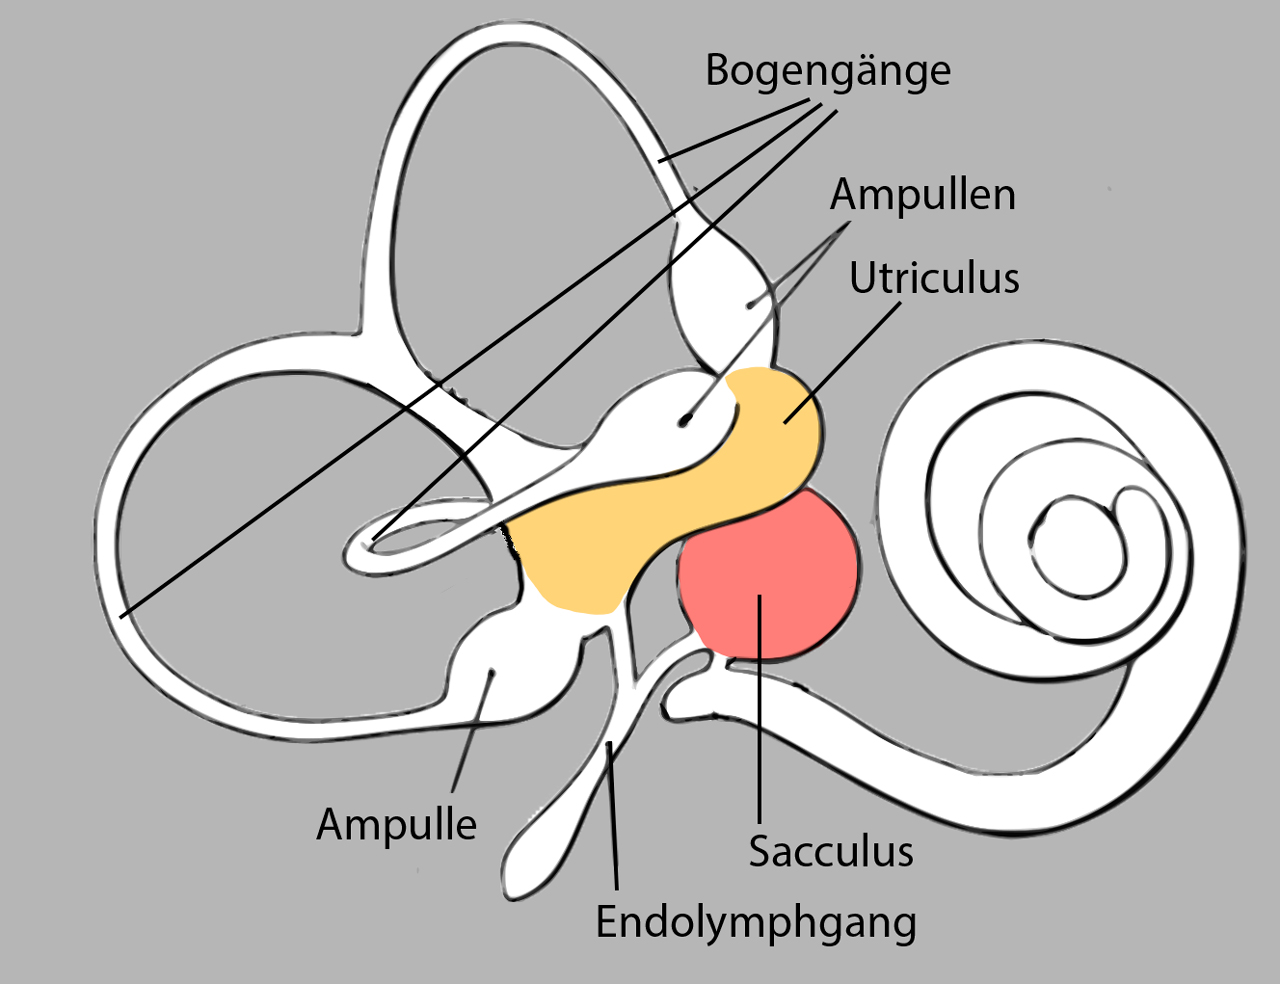
\includegraphics[scale=0.2]{pics/vestibular-system.jpg}
    \caption{Vestibuläres System}
    \label{fig:cybersickness:vestibular-system}
\end{figure}

Das Gleichgewichtssystem, auch vestibuläres System genannte, befindet sich im Innenohr und ist für die Wahrnehmung von Bewegung  und Orientierung im Raum verantwortlich. Es besteht aus drei Bogengängen, die Drehbewegungen des Kopfes erfassen, sowie dem Utriculus und dem Sacculus, die lineare Beschleunigungen und die Lage zur Schwerkraft registrieren. Gemeinsam liefern sie dem Gehirn Informationen darüber, wie sich der Kopf - und damit der Körper - im Raum bewegt.

\subsection{Das Visuelle System}
Dieses eben erwähnte Gleichgewichtssystem arbeitet eng mit dem visuellen System zusammen. Während die Augen visuelle Eindrücke von Bewegung liefern, sorgt das vestibuläre System dafür dass die tatsächlichen Bewegungen des Kopfes erkannt und ausgeglichen werden. Diese geschieht unter anderem durch den sogenannten vestibulo-okulären Reflex, der die Augen stabilisiert, wenn sich der Kopf bewegt. (QUELLE2)

Stimmen die Signale von Auge und Gleichgewichtssystem jedoch nicht überein, kann eine Sinnestäuschung entstehen. So kann man sich beispielsweise auch ohne tatsächliche Bewegung bewegt fühlen, wenn sich das Sichtfeld verändert. Dieser Effekt wird als Vection bezeichnet. Solche Wahrnehmungskonflikte zwischen Augen und Gleichgewichtssinn sind eine zentrale Ursache für Cybersickness, also die Übelkeit oder Desorientierung, die in virtuellen Umgebungen auftreten kann.

\section{Ursachen für Cybersickness in der virtuellen Realität}
Nachdem geklärt wurde, auf welche zwei wichtigen biologischen Faktoren die Cybersickness in der echten Welt zurückzuführen ist, muss nun untersucht werden, warum die Symptome beim Verwenden einer VR-Software auftreten.
Die Ursachen für Cybersickness werden unter anderem durch die \emph{Sensory Conflict Theory} (Theorie des sensorischen Konflikts), die \emph{Poison Theory} (Vergiftungshypothese) und die \emph{Postural Instability Theory} (Theorie der posturalen Instabilität) beschrieben (QUELLE4).

\subsection{Sensory Conflict Theory}
Die Sensory-Conflict-Theorie gilt als die älteste und am weitesten akzeptierte Erklärung für Cybersickness.(QUELLE5QUELLE2) Demnach wird Cybersickness durch Diskrepanzen zwischen den für die Wahrnehmung von Bewegung und Orientierung zuständigen Sinnen ausgelöst. Besonders relevant ist dabei der Konflikt zwischen dem visuellen und dem vestibulären System. (SIEHE KAPITEL DAS GLEICHGEWICHTSSYSTEM) Tritt eine Situation auf, in der das visuelle System signalisiert, das vestibuläre System jedoch keine entsprechende physische Bewegung registriert, entsteht ein wahrnehmungsbasierter Konflikt, den der Körper nicht korrekt verarbeiten kann.

Ein typisches Beispiel hierfür ist ein virtueller Fahrsimulator: Während der Nutzer visuell die Bewegung auf der Straße und das Vorbeiziehen von Gebäuden wahrnimmt, bleibt sein Körper statisch. Da das vestibuläre System keine Informationen über Beschleunigung oder Drehungen liefert, entsteht ein Mismatch der Sinneseindrücke, das Cybersickness hervorrufen kann. Diese Theorie wird durch zahlreiche Studien unterstützt.(QUELLE6QUELLE7) Sie betont die zentrale Rolle des visuell-vestibulären Konflikts, weist jedoch auch Einschränkungen auf: So kann sie beispielsweise nicht zuverlässig vorhersagen, wer unter Cybersickness leidet oder wie stark die Symptome ausfallen. Auch erklärt sie nicht vollständig, warum manche Personen empfindliche reagieren als andere. 

\subsection{Poison Theory}
Die Poison-Theorie versucht, die Entstehung von Cybersickness aus evolutionärer Sicht zu erklären.(QUELLE8) Demnach dienen Übelkeit und Erbrechen ursprünglich als Schutzmechanismus, um den Körper vor aufgenommenen Giften zu warnen und diese aus dem Magen zu entfernen. Bei Cybersickness kann die inadäquate Stimulation der visuellen und vestibulären Systeme dazu führen, dass der Körper die Sinneseindrücke falsch interpretiert und glaubt, eine giftige Substanz aufgenommen zu haben. Dadurch treten Symptome wie Übelkeit auf.(QUELLE2QUELLE5)

Einige Studien(QUELLE9QUELLE10) unterstützen diese Hypothese und zeigen, dass die Symptome in sehr spezifischen Situationen reduziert werden können. Dennoch ist die Theorie umstritten, da sie kaum Vorhersagekraft hat und nicht erklärt, warum manche Personen bei identischen Reizen in virtuellen Umgebungen Cybersickness entwickeln, andere jedoch nicht. Zudem erscheint der zeitliche Ablauf evolutionär problematisch, da Toxine zu lange brauchen würden, um die vestibulären Mechanismen auszulösen, sodass Erbrechen nicht effektiv wäre. Daher ist die Validität der Theorie bislang schwer nachzuweise. Sie wird eher als interessante Hypothese betrachtet, die bei der Gestaltung von VR-Erfahrungen vorsichtig berücksichtigt werden sollte.

\subsection{Postural Instability Theory}
Die von Ricco und Stoffregen entwickelte Postural-Instability-Theorie besagt, dass Cybersickness durch anhaltende Haltungsinstabilität entstehen. Der Mensch strebt danach, seine posturale Stabilität aufrechtzuerhalten, das heißt, einen Zustand zu erreichen, in dem unkontrollierte Bewegungen des Wahrnehmungs- und Handlungssystems minimiert sind. Verändern sich die Umweltbedingungen abrupt oder fehlen geeignete Strategien zur Haltungsanpassung, kann die Kontrolle über die Körperhaltung vorübergehend verloren gehen.(QUELLE11), (QUELLE5QUELLE2)

Laut dieser Theorie tritt Cybersickness auf, wenn über längere Zeiträume posturale Instabilität besteht. Die Schwere der Symptome hängt dabei direkt von der Dauer dieser Instabilität ab. In virtuellen Umgebungen entsteht diese Instabilität häufig, weil die visuell dargestellten Bewegungen oder Beschleunigungen nicht mit den tatsächlichen körperlichen Bewegungen übereinstimmen. Dadurch werden herkömmliche Strategien zur Stabilisierung der Körperhaltung unwirksam.(QUELLE11)

Ricco und Stoffregen ordnen Cybersickness der Kategorie "altered specificity" zu, also Situationen, in denen optische Reize nicht mehr eindeutig mit realen Umweltbedingungen verknüpft sind. Die Theorie wurde als Alternative zur Sensory-Conflict-Theorie entwickelt. Sie argumentiert., dass nicht sensorische Konflikte, sondern der Verlust posturaler Kontrolle die eigentliche Ursache von Cybersickness sei.(QUELLE11QUELLE2)

\subsection{Festlegung der Theorie zur Reduzierung der Cybersickness für die Hardware-Komponente}

Es wurden diverse Studien (QUELLE11) zur Glaubhaftigkeit dieser Theorie durchgeführt. Die Ergebnisse dieser Studien deuten darauf hin, dass in disesm nur ein schwacher Zusammenhang zwischen Haltungsinstabilität und Cybersickness festgestellt werden konnte.

Da Cybersickness durch diese drei Theorien definiert wird, von denen zwei - die Poison-Theorie und die Postural-Instability-Theorie - teilweise widerlegt bzw. durch Experimente angezweifelt wurden (SIEHE 3.3.2 AS 2, QUELLE11), wurde im Rahmen diese Projekts der Fokus bei der Hardware-Komponente der Simulation, deren wichtige Aufgabe es unter anderem ist, die Cybersickness zu reduzieren, auf die Sensory-Conflict-Theorie gelegt.

\section{Reduzierung der Cybersickness}
\setauthor{Linnea Schönbauer}

\section{Hardware Prototyp}
\setauthor{Linnea Schönbauer}
